\section*{Problem 4: A Better Circulator}
\addcontentsline{toc}{section}{Problem 4: A Better Circulator}

The scattering parameter matrix is given in the following form:

\[ 
    S_{circ} = \begin{pmatrix}
        0 & a & b \\ b & 0 & a \\ a & b & 0
    \end{pmatrix} 
\]

where $ a = .03$ and $b = .93$. This problem will be broken up into different
stages considering the different paths the wave will follow. First, the
incident wave $V_{in}$ will encounter the first circulator. Because $S_{3,1}$ is
nonzero, some of the wave ( $V_3 = a V_{in}$ ) will head down towards a second
circulator. This wave will travel into the first port of that circulator and out
of the second port $V_{RF_3} = a b V_{in}$. The wave that traveled out of the
second port of the first circulator will travel towards its second circulator.
Some of that wave will travel through port three of the rightmost circulator
$V_{RF_5} = b a V_{in}$. Now, we have to consider exactly how both waves
interact at ports 2 and 3 to combine to give the wave at port 4 ($V_{RF_7}$).

The ideal 180\degree~coupler has the following scattering parameters:

\[
    S_{180 \degree} = \frac{-j}{\sqrt{2}} \begin{pmatrix}
        0 & 1 & 1 & 0 \\ 1 & 0 & 0 & -1 \\ 1 & 0 & 0 & 1 \\ 0 & -1 & 1 & 0
    \end{pmatrix}
\]

Thus, the wave incident at port 2 will contribute to a wave at port 4 that is
180\degree~out of phase with respect to that incident wave. The wave at port 3
will give rise to a wave at port 4 that is in phase with that incident wave.
Thus:

\[ 
    V_{RF_7} = -V_{RF_3} + V_{RF_5} = -a b V_{in} + a b V_{in} = 0
\]

Thus, even though the circulator is not ideal, the three-port device formed by all of
these devices is ideal. However, it's worth noting that this result assumes the
rat race coupler is ideal (balanced) such that the waves perfectly cancel.
Practically, this will not occur and the non-idealities of the circulator have
to be compared to the non-idealities of the rat race coupler.

\begin{figure}[H]
    \centering
    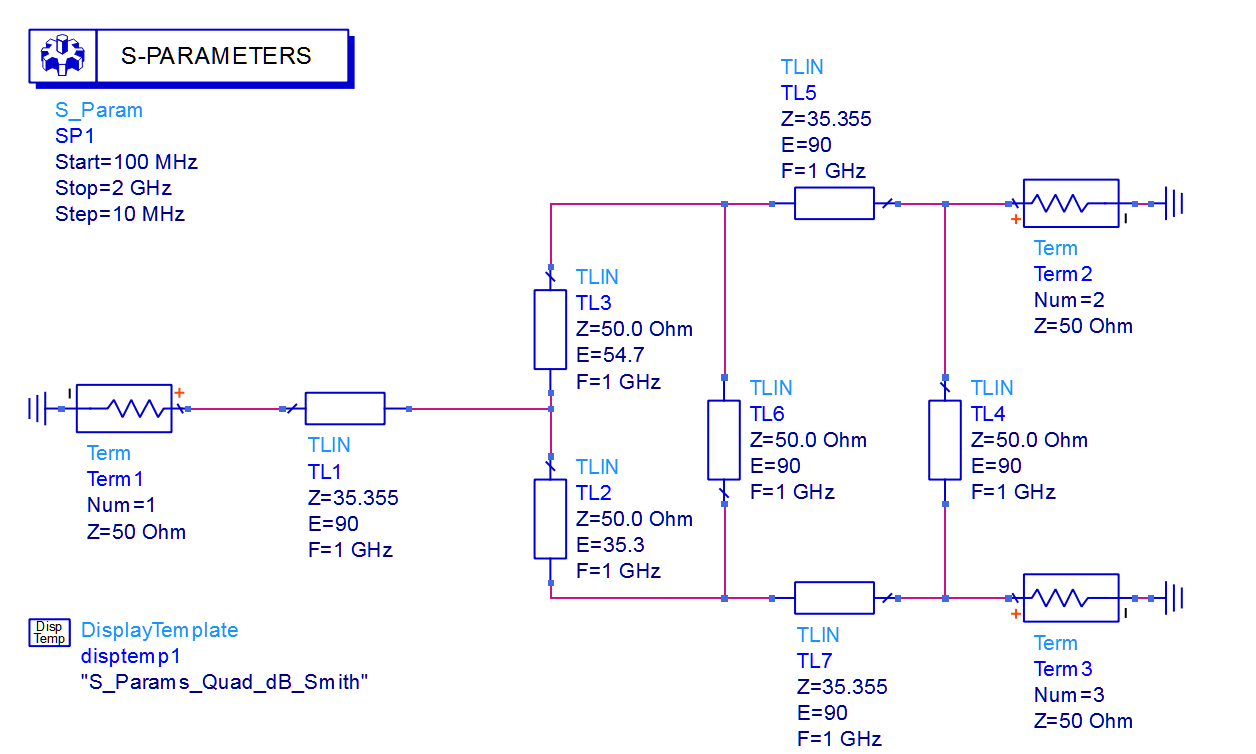
\includegraphics[width=0.8\linewidth]{img/Problem3/PowerSplitterSchematic.PNG}
    \caption{Schematic for the Power Splitter}
    \label{fig:img/Problem3/PowerSplitterSchematic}
\end{figure}
